\usepackage{etex} %эта магическая херь избавляет от переполнения регистров TeX а!!!

\mode<article>{\usepackage{fullpage}}
\mode<presentation>{
    \usetheme{Madrid}
    \useoutertheme{shadow}
} 

\usepackage[utf8]{inputenc}
\usepackage[russian]{babel}
\usepackage{indentfirst}
\usepackage{graphicx}

\usepackage{amsmath}
\usepackage{amsfonts}
\usepackage{amsthm}
%\usepackage{algorithm}
%\usepackage{algorithmic}

%\usepackage[all]{xy}

\date{Лекция по дисциплине <<методы и средства защиты компьютерной информации>> (\today)}
\author[М.~М.~Шихов]{Михаил Шихов \\ \texttt{\underline{m.m.shihov@gmail.com}}}

%%для рисования графов пакетом xy-pic
%\entrymodifiers={++[o][F-]}

%%для псевдокода алгоритмов (algorithm,algorithmic)
%\renewcommand{\algorithmicrequire}{\textbf{Вход:}}
%\renewcommand{\algorithmicensure}{\textbf{Выход:}}
%\renewcommand{\algorithmiccomment}[1]{// #1}
%\floatname{algorithm}{Псевдокод}

%\setbeamercolor{alerted text}{fg=-green} %gyan, blue, green, -green

\title[Контроль доступа]{Контроль доступа}


\begin{document}


%титул и содержание статьи
\mode<article>{\maketitle\tableofcontents}

%титул и содержание презентации
\frame<presentation>{\titlepage}
\begin{frame}<presentation>[allowframebreaks]
    \frametitle{Содержание}\tableofcontents
\end{frame}


\section{Контроль доступа}


\begin{frame}
\frametitle{Монитор доступа}
\begin{figure}
    \begin{center}
        \mode<presentation>{ 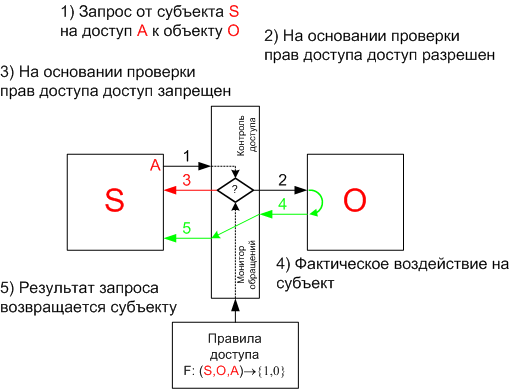
\includegraphics[height=.7\textheight]{pict/AccessControl} }
        \mode<article>{ 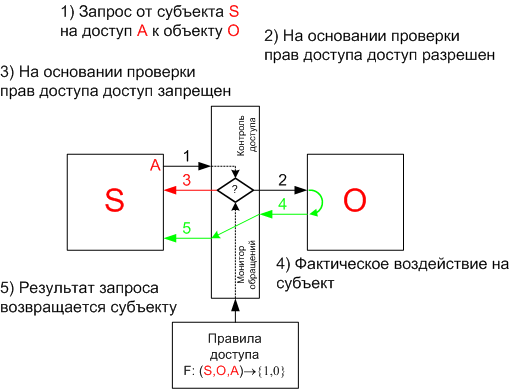
\includegraphics[width=.7\textwidth]{pict/AccessControl} } 
        \caption{Монитор доступа}\label{pict:AccessControl}
    \end{center}
\end{figure} 
\mode<article>{см. рис. \ref{pict:AccessControl}}
\end{frame}


\begin{frame}
\frametitle{Контроль доступа}
\begin{definition}%theorem, lemma, proof, corollary, example
    \alert{Основная теорема безопасности}: если начальное состояние системы безопасно и все переходы системы из
    состояния в состояние не нарушают накладываемых на них ограничений, то любое состояние системы безопасно.
\end{definition}
Различают следующие модели систем контроля доступа.
\begin{itemize}
    \item Discretionary access control (DAC). Дискреционные или избирательные.
    \item Mandatory access control (MAC). Мандатные или полномочные.
    \item Role-based access control (RBAC). Ролевые. 
\end{itemize}
\end{frame}

%TODO авторизация

\section{Формальные модели безопасности}

Формальные модели безопасности на основе дискретных компонент могут рассматриваться как математическое обобщение систем контроля доступа. Эти понятия практически тождественны и их разделяют на такие же классы: Дискреционные (Discretionary / DAC), Мандатные (Mandatory / MAC), Ролевые (Role Based / RBAC). 
Формальные модели используются в следующих случаях.
\begin{itemize}
    \item В качестве эталона.
    \item При составлении формальной спецификации политики безопасности.
    \item При формальном подтверждении свойств разрабатываемой системы безопасности.
\end{itemize}


\subsection{DAC}

Данной моделью описываются рассмотренные выше дискреционные системы контроля доступа DAC.  
Выделяют множества активных сущностей субъектов ($S$), пассивных объектов ($O$) и прав доступа субъекта к объекту ($R$). Множества прав доступа определяет полномочия на выполнение соответствующих действий субъекта над объектом. Важно также отметить, что $S\subset O$. Пространство состояний системы описывается декартовым произведением $O\times S\times R$. Текущее состояние системы $Q$ в этом пространстве определено тройкой, состоящей из множества субъектов, множества объектов и матрицы доступа $M$: $Q=(S, O, M)$. Строки матрицы доступа соответствуют субъектам, столбцы --- объектам, а элементы матрицы $M[s,o]\subset R, s\in S, o\in O$.


\begin{frame}
    \frametitle{Модель Харрисона-Руззо-Ульмана}
    \framesubtitle{DAC. HRU --- Harrison-Russo-Ullman}
    
    Введем обозначения:
    \begin{itemize}
        \item $O$ --- множество объектов;
        \item $S$ --- множество субъектов, $S\subset O$;
        \item $R$ --- множество прав доступа субъекта к объекту;
        \item $M$ --- матрица доступа, $M[s,o]\subset R, s\in S, o\in O$;
        \item $Q$ --- состояние системы, $Q=(S, O, M)$.
    \end{itemize}
    Пространство состояний: $O\times S\times R$.
\end{frame}


\begin{frame}
    \frametitle{Модель Харрисона-Руззо-Ульмана}
    \framesubtitle{Элементарные операции}
    
    \begin{itemize}
        \item enter $r$ into $M[s, o]$. \mode<article>{Добавить субъекту $s$ право на действие $r$ над объектом $o$.}
        \item delete $r$ from $M[s, o]$. \mode<article>{Отнять у субъекта $s$ право на действие $r$ над объектом $o$.}
        \item create subject $s$. \mode<article>{Создать субъект.}
        \item create object $o$. \mode<article>{Создать объект.}
        \item destroy subject $s$. \mode<article>{Удалить субъект.}
        \item destroy object $o$. \mode<article>{Удалить объект.}
    \end{itemize}
\end{frame}


\begin{frame}
    \frametitle{Модель Харрисона-Руззо-Ульмана}
    \framesubtitle{Команды}
    
    \[
        \alpha(x_1,\ldots,x_k)=
        \text{if}
        \left(
            \begin{array}[c]{c}
                r_1 \text{\,in\,} M[x_{s_1},x_{o_1}] \& \\
                \cdots \\
                \& r_m \text{\,in\,} M[x_{s_m},x_{o_m}]
            \end{array}
        \right)
        \text{\,then\,} op_1,\ldots,op_n,
    \]
    где $x_1,\ldots,x_k$ --- аргументы команды ($x_i\in(S\cup O)$), $op_1,\ldots,op_n$ набор элементарных операций,
    которые выполняются как одно целое, если условие в скобках истинно и не выполняются в противном случае.
\end{frame}


\begin{frame}
    \frametitle{Модель Харрисона-Руззо-Ульмана}
    \framesubtitle{Формальное определение}
    $\sum(Q_0,R,C)$
    \begin{itemize}
        \item $Q_0=(S_0, O_0, M_0)$ --- исходное состояние.
        \item $R$ --- множество прав доступа субъекта к объекту;
        \item $C$ --- множество команд вида $\alpha(x_1,\ldots,x_k)$.
    \end{itemize}
    Переход к новому состоянию происходит при выполнении команды из множества команд: $Q_n\xrightarrow{C_n}Q_{n+1}$
\end{frame}


\begin{frame}
    \frametitle{Модель Харрисона-Руззо-Ульмана}
    \framesubtitle{Теорема безопасности}
    
    \begin{definition}%theorem, lemma, proof, corollary, example
        \alert{Основная теорема безопасности для HRU}: Для заданной системы начальное состояние $Q_0=(S_0, O_0, M_0)$
        является безопасным относительно права $r$, если не существует применимой к $Q_0$ последовательности команд,
        в результате выполнения которой право $r$ будет добавлено в ячейку матрицы $M$, в которой оно отсутствовало в
        состоянии $Q_0$.
    \end{definition}

    \mode<article> {
        Для того, чтобы доказать за конечное время критерий безопасности модели она должна удовлетворять одному из 
        следующих свойств (сформулированы и доказаны авторами модели).
    }
    
    \begin{enumerate}
        \item Команды должны состоять не более чем из одной элементарной операции.
        \item Команды должны содержать не более одного условия и не должны содержать операций destroy и delete.
        \item Команды не должны содержать операций create.
    \end{enumerate}
\end{frame}


\begin{frame}
    \frametitle{Подверженность DAC атакам троянского коня}
    \framesubtitle{Начальное состояние системы}
    
    \begin{enumerate}
        \item $R=\{rd,wr,exec,own\}$
        \item $Q_0=(S_0, O_0, M_0)$, $S_0=\{A,C\}$, $O_0=\{A,C,F\}$
        \[
            M_0=
            \begin{array}[c]{c|ccc}
                    & A     &  C    &  F            \\ \hline
                A   &       &       &  \{rd,wr,own\}\\ 
                C   &       &       &               \\ 
            \end{array}
        \]
        \item $C$
        \begin{enumerate}
            \item makeObj($s$,$o$)=if(true) then create object $o$, enter $own$ into $M[s,o]$.
            \item setExec($s_o$,$s$,$o$)=if($own$ in $M[s_o,o]$) then enter $exec$ into $M[s,o]$.
            \item\ldots
        \end{enumerate}
    \end{enumerate}
    Злоумышленник $C$ желает получить доступ к файлу $F$, который ему не принадлежит.
\end{frame}


\begin{frame}
    \frametitle{Подверженность DAC атакам троянского коня}
    \framesubtitle{Атака}
    
    \begin{enumerate}
        \item makeObj($C$,$T$). $C$ создает троянскую программу $T$.
        \item setExec($C$,$A$,$T$). $C$ дает право $A$ на запуск $T$.
        \item \label{ert:exec}$C$ провоцирует запуск $T$ субъектом $A$.
            После чего матрица доступа будет выглядеть так:
        \[
            M_{\ref{ert:exec}}=
            \begin{array}[c]{c|cccc}
                      & A   & C & F             & T       \\ \hline
                A     &     &   & \{rd,wr,own\} & \{exec\}    \\ 
                C     &     &   &               & \{own\}     \\ 
                T_A   &     &   & \{rd,wr,own\} & \{exec\}    
            \end{array}
        \]        
        \item От логики работы троянской программы, ставшей процессом (субъектом) $T_A$, зависит будущее $F$.
    \end{enumerate}
\end{frame}


Хранить матрицу доступа $M$ целиком нецелесообразно ввиду её разреженности, поэтому хранят.
\begin{itemize}
    \item Вместе с объектом $o$ список $\langle s_1\to M[s_1,o],\ldots,s_N\to M[s_N,o]\rangle$. 
        Такой список называется списком контроля доступа (ACL --- Access Control List).
    \item Вместе с субъектом $s$ список $\langle o_1\to M[s,o_1],\ldots,o_N\to M[s,o_N]\rangle$. 
        Такой список называется перечнем возможностей (Capability List, C-List).
\end{itemize}
Получить доступ к этим элементам, минуя монитор обращений, невозможно. То есть они находятся (доступны) только из режима ядра. Пустые ячейки матрицы $M$ в списках не сохраняются $M[s,o]\neq\emptyset$.


\begin{frame}<presentation>
    \frametitle{Списки доступа и перечни возможностей}
    Матрица доступа $M$ разрежена и обычно используются <<срезы>> прав доступа по субъектам или объектам.
    \begin{itemize}
        \item ACL. $o\to\langle s_1\to M[s_1,o],\ldots,s_N\to M[s_N,o]\rangle$. 
            Список контроля доступа (ACL --- Access Control List). $M[s_i,o]\neq\emptyset$.
        \item C-List. $s\to\langle o_1\to M[s,o_1],\ldots,o_N\to M[s,o_N]\rangle$. 
            Перечень возможностей (C-List --- Capability List). $M[s,o_i]\neq\emptyset$.
    \end{itemize}
    
    Эти списки и перечни недоступны прикладному коду. Доступ косвенный и только через монитор обращений.
\end{frame}

Перечни возможностей, например хранятся в метаданных процесса (субъекта), когда он уже получил доступ к объекам. Часто эти схемы работают совместно. Например, процесс открывает файл (указывая какие операции он намерен производить над файлом), и система контроля доступа по ACL списку файла проверяет разрешен ли доступ. Если доступ разрешен, то процессу возвращается дескриптор файла с ассоциированным с ним списком прав на данный объект. Далее, при обращениях к файлу через дескриптор, проверка по уже ACL не осущетвляется (так как это потребует больших затрат времени). Список дескрипторов объектов с ассоциированными правами доступа можно считать перечнем возможностей процесса.

Аналогом перечня возможностей, используемого в распределенных системах, являются, например, маркеры доступа протокола аутентификации Cerberos.


\begin{frame}
    \frametitle{DAC. Итоги}
    \begin{itemize}
        \item Все субъекты и объекты системы должны быть идентифицированы.
        \item Права доступа субъекта к объекту системы определяются на основании некоторого внешнего по отношению к системе правила (свойство избирательности).
        \item Главный принцип: что не разрешено --- то запрещено.
        \item Пользователь должен обладать дополнительными знаниями об особенностях системы безопасности.
        \item Поверженность атакам <<троянского коня>>.
        \item Широко используется в коммерческом секторе.
    \end{itemize}
\end{frame}


\subsection{MAC}

\begin{frame}
    \frametitle{Модель Бела-Ла Падулы}
    
    \begin{itemize}
        \item Задан линейно упорядоченный набор уровней безопасности.
        \item Процесс, запущенный на уровне безопасности $k$, может выполнять:
        \begin{itemize}
            \item Чтение из объектов $o$ с уровнем безопасности $l_o\leq k$.
            \item Запись в объекты $o$ с уровнем безопасности $l_o\geq k$.
        \end{itemize}
    \end{itemize}
    
    Модель Бела-Ла Падулы разработана для обеспечения \alert{конфиденциальности}, гарантий \alert{целостности} она не дает.\mode<article>{Например, лейтенантскйй процесс может переписать генеральский файл, но прочитать его не может.}
\end{frame}


\begin{frame}
\frametitle{Модель Бела-Ла Падулы}
\begin{figure}
    \begin{center}
        \mode<presentation>{ 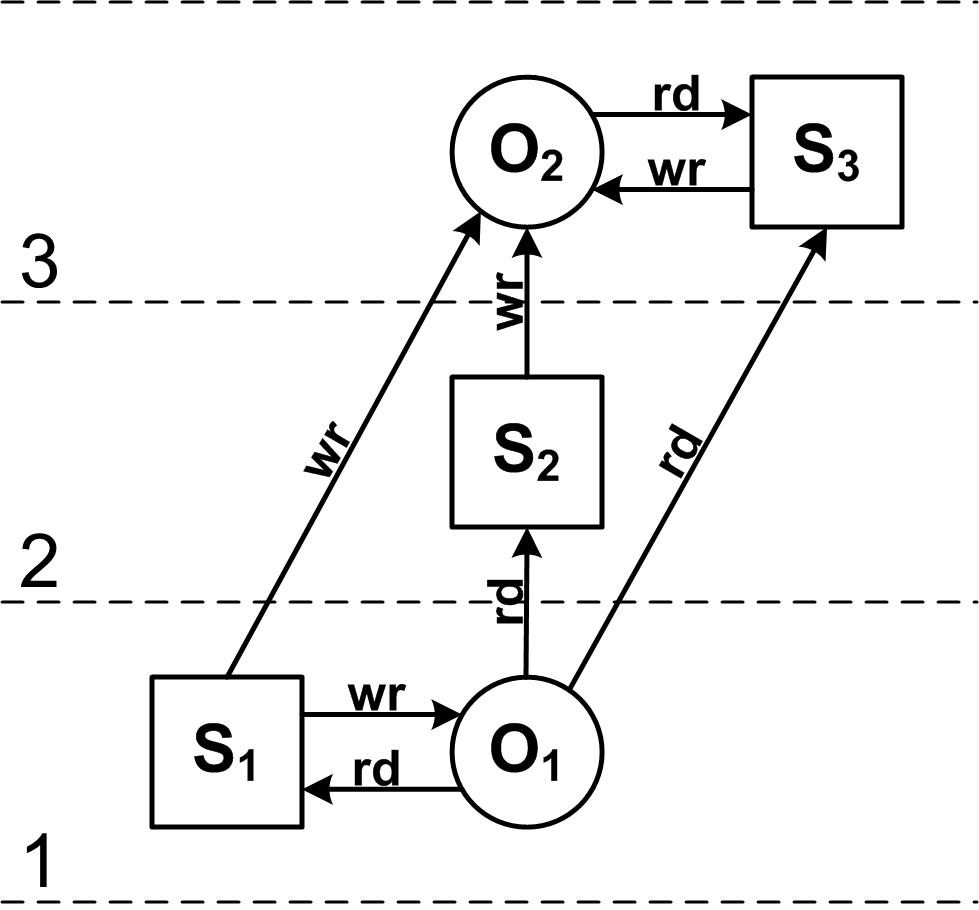
\includegraphics[height=.7\textheight]{pict/lapadula} }
        \mode<article>{ 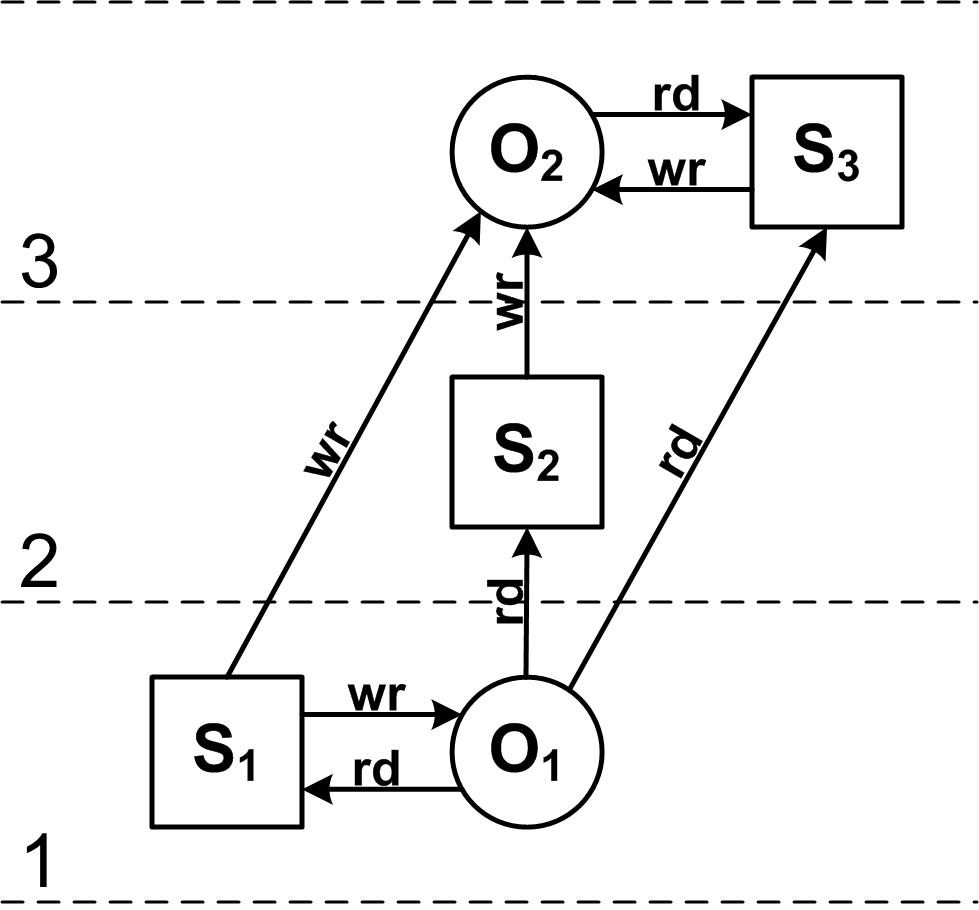
\includegraphics[width=.7\textwidth]{pict/lapadula} } 
        \caption{Модель Бела-Ла Падулы}\label{pict:lapadula}
    \end{center}
\end{figure} 
\mode<article>{см. рис. \ref{pict:lapadula}}
\end{frame}


\begin{frame}
    \frametitle{Модель Биба}
    
    \begin{itemize}
        \item Задан линейно упорядоченный набор уровней безопасности.
        \item Процесс, запущенный на уровне безопасности $k$, может выполнять:
        \begin{itemize}
            \item Запись в объекты $o$ с уровнем безопасности $l_o\leq k$.
            \item Чтение из объектов $o$ с уровнем безопасности $l_o\geq k$.
        \end{itemize}
    \end{itemize}
    
    Модель Биба разработана для обеспечения \alert{целостности}, гарантий \alert{конфиденциальности} она не дает.\mode<article>{Например, лейтенантскйй процесс не может переписать генеральский файл, но может его прочитать}
\end{frame}


\begin{frame}
\frametitle{Модель Биба}
\begin{figure}
    \begin{center}
        \mode<presentation>{ 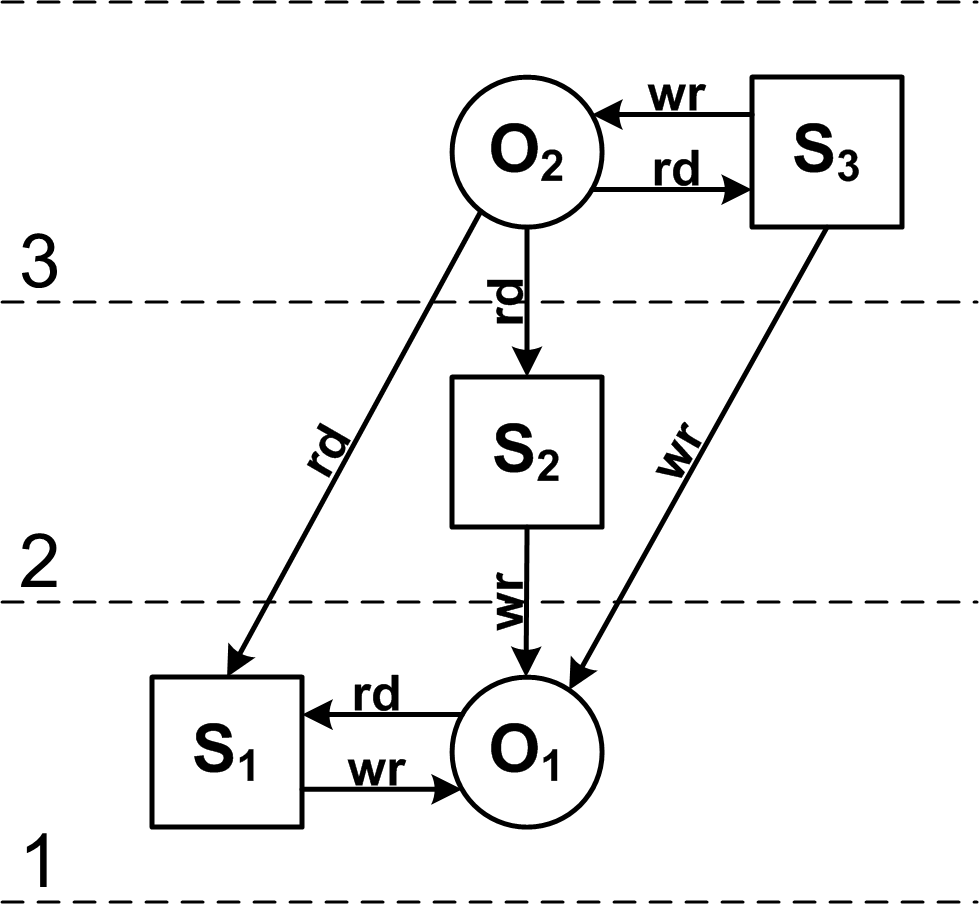
\includegraphics[height=.7\textheight]{pict/biba} }
        \mode<article>{ 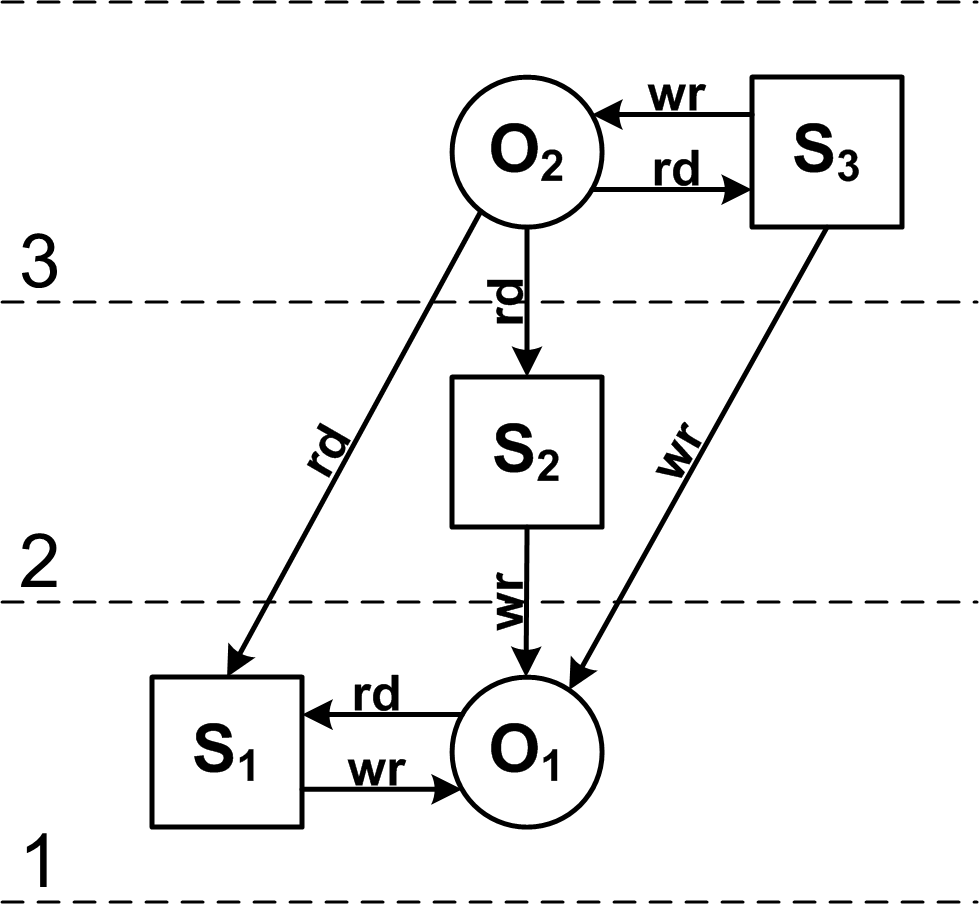
\includegraphics[width=.7\textwidth]{pict/biba} } 
        \caption{Модель Биба}\label{pict:biba}
    \end{center}
\end{figure} 
\mode<article>{см. рис. \ref{pict:biba}}
\end{frame}


\begin{frame}
    \frametitle{MAC. Итоги}
    \begin{itemize}
        \item Все субъекты и объекты системы должны быть однозначно идентифицированы.
        \item Должен быть задан линейно упорядоченный набор уровней безопасности.
        \item Высокая степень надежности, правила ясны и понятны.
        \item Проблема <<слепой>> записи.
        \item Только два типа доступа и соответственно два типа потоков информации (чтение $s\xleftarrow{rd}o$ и запись $s\xrightarrow{wr}o$).
        \item Широко используется в военном и оборонном секторах.
    \end{itemize}
\end{frame}


\subsection{RBAC}

\begin{frame}
    \frametitle{Ролевая модель}
    \begin{definition}
        \alert{Роль} --- абстрактный субъект, с которым связан ограниченный и логически связанный набор \alert{полномочий},
            необходимых для осуществления необходимой дятельности.
    \end{definition}

    \begin{itemize}
        \item Основана на HRU.
        \item Вводится понятие \alert{сеанса} работы.
        \item Дополнительно вводятся правила, регламентирующие назначение ролей пользователям и их активацию во время сеансов.
    \end{itemize}
\end{frame}


Далее следует обратить внимание, что речь об \emph{объектах} не идет! Роль определяет \emph{полномочия} то есть контроль доступа может осуществляться как в мандатной модели (например, полномочие <<первый уровень безопасности>>, <<доступ ко всем таблицам>>, <<администрирование>>, <<работа с принтерами>>, <<настройка сети>>). Полномочиями может являться и полный \emph{перечень возможностей} (см. выше). Обычно группам раздаются права на основе матрицы доступа, как в дискреционной модели.

\begin{frame}
    \frametitle{Ролевая модель}
    \frametitle{Формальное определение}
    
    \begin{itemize}
        \item $U$ --- множество пользователей.
        \item $R$ --- множество ролей.
        \item $P$ --- множество полномочий.
        \item $S$ --- множество сеансов работы пользователей с системой.
        \item $PA\subseteq P\times R$ --- отображение множества полномочий на множество ролей. 
        \item $UA\subseteq U\times R$ --- отображение множества пользователей на множество ролей. 
        \item $user:S\to U$ --- функция определяющая пользователя для каждого сеанса.
        \item $roles:S\to \mathcal{P}(R)$ --- функция определяющая набор ролей для каждого сеанса: $roles(s)=\{r_i|(user(s),r_i)\in UA\}$.
        \item $perms:S\to \mathcal{P}(P)$ --- функция определяющая набор полномочий для каждого сеанса: $perms(s)=\bigcup_{r\in roles(s)} \{p_i|(p_i,r)\in PA\}$.
    \end{itemize}
\end{frame}


Порой могут возникнуть неоднозначности, если пользователь входит в несколько групп:

\begin{frame}
    \frametitle{Варианты реализации RBAC на ACL}
    \begin{table}[ht]
        \caption{Варианты реализации RBAC на ACL}\label{t:rbacOnAcl}
        \centering
        \begin{tabular}[c]{|l|l|l|l|}
            \hline\hline
            Запрос & Сеанс              & Объект                                               & Доступ   \\
            \hline\hline
            r      & $s\to\{R_2\}$      & $o\to\langle R_1\to\bar{r}\bar{w},R_2\to rw \rangle$ & Разрешен \\ 
            \hline
            x      & $s\to\{R_2\}$      & $o\to\langle R_1\to\bar{r}\bar{w},R_2\to rw \rangle$ & Запрещен \\ 
            \hline
            w      & $s\to\{R_1\}$      & $o\to\langle R_1\to\bar{r}\bar{w},R_2\to rw \rangle$ & Запрещен \\ 
            \hline
            r      & $s\to\{R_1,R_2\}$  & $o\to\langle R_1\to\bar{r}\bar{w},R_2\to rw \rangle$ & ???      \\ 
            \hline
        \end{tabular}
    \end{table}
    \mode<article>{См. таблицу \ref{t:rbacOnAcl}}
\end{frame}


\begin{frame}
    \frametitle{RBAC. Итоги}
    \begin{itemize}
        \item Все, что справедливо для DAC.
        \item Роли соответствуют трудовым функциям пользователя в АИС.
        \item Проще в управлении, чем DAC.
        \item Приближены к MAC в силу жесткости правил контроля.
        \item Активно используются в коммерческом секторе.
    \end{itemize}
\end{frame}


\section{Примеры систем контроля доступа}


\subsection{ОС Unix/Linux}


\begin{frame}
    \frametitle{Unix, Linux}
    \framesubtitle{Субъекты защиты}
    Пользователь (UID) может входить в несколько групп (GID) одновременно. Процесс в *nix содержит следующие атрибуты.
    \begin{itemize}
        \item PID --- идентификатор процесса.
        \item PPID --- идентификатор родительского процесса.
        \item Nice Number --- приоритет процесса.
        \item TTY --- терминал, ассоциированный с процессом (демон не имеет TTY).
        \item RID(RUID),EUID --- реальный и эффективный идентификаторы пользователя.
        \item RGID,EGID --- реальный и эффективный идентификаторы группы.
    \end{itemize}
    Имеется суперпользователь (\alert{root}), для которого \alert{нет} ограничений.
\end{frame}


Многие сущности в Linux рассматриваются как файл, а иногда и отображаются на файловую систему. Объекты межпроцессного взаимодействия также рассматриваются как файлы. По крайней мере на уровне программного интерфейса работа с ними напоминает работу с файлом. Права доступа к ним аналогичны правам доступа к файлу, например, разделяемая между процессами память будет рассматриваться как файл с аналогичными правами доступа.

\begin{frame}
    \frametitle{Unix, Linux}
    \framesubtitle{Объекты защиты}
    
    Для каждого объекта можно определить владельца-пользователя (UID) и владельца-группу (GID). Выделяют три класса доступа в отношении каждого объекта (файла).
    \begin{itemize}
        \item User access (\alert{u}) --- в отношении владельца-пользователя объекта.
        \item Group access (\alert{g}) --- в отношении владельца-группы объекта.
        \item Other access (\alert{o}) --- в отношении остальных пользователей (кроме root).
    \end{itemize}
    Для каждого класса поддерживается три основных типа прав доступа: чтение(\alert{r}), запись(\alert{w}), выполнение(\alert{x}) и ряд дополнительных (например, права \alert{s},\alert{t} см. далее).
    
    Базовая концепция: <<все есть файл>>. На файловую систему отображаются, например, такие объекты как блочные и символьные устройства, именованные каналы и т.д. 
\end{frame}


В листинге команды \verb"ls -l" отображающей содержимое текущего каталога, для файлов и каталогов права доступа отображаются строкой из 10-и символов: \verb"X XXX XXX XXX".
    
Первый символ --- тип файла (например: каталог (\verb"d"), просто файл(\verb"-"), символьная ссылка(\verb"l"),  файл блочного устройства(\verb"b"), и т.д.).
    
Следующие три группы из трех символов определяют права в отношении владельца-пользователя, владельца-гуппы и всех остальных соответственно.

\begin{frame}[fragile]
    \frametitle{Unix, Linux}
    \framesubtitle{ls -l}

\begin{verbatim}
-rw-r--r-- 1 user1 group1 120   Dec 22 19:30 main.cpp
drwxr-xr-- 2 user1 group1 64    Dec 22 11:20 folder
-rwxr-xr-- 2 user1 group1 4801  Dec 22 19:31 main.exe
\end{verbatim}

Чтобы файл стал программой, необходимо добавить право на выполнение (\alert{x}) в соответствующий класс доступа.

Бинарные файлы программ (например, ELF) содержат сигнатуру, а текстовые скрипты обычно первой строкой содержат:

\verb"#!/path/to/interpreter"

\end{frame}


Файл является исполнимым если у него есть право на выполнение. Это значит, что является ли файл программой зависит не о расширения файла, а от соответствующего права. Бинарные файлы ELF, COFF содержат в заголовке специальные сигнатуры. Текстовые исполнимые файлы-скрипты, обычно содержат в самом начале строку \verb"#!/path/to/interpreter".

В отношении каталогов право на выполнение дает возможность читать метаданные файла, а также переходить в каталог. Право на чтение позволяет получить лишь список имен файлов данного каталога. Можно создать <<темную комнату>> для запретив чтение, но разрешив выполнение для каталога. Право записи позволяет создавать или удалять в каталоге файлы.

Командой \verb"chmod +t directory" можно запретить удаление тех файлов каталога directory, в отношении которых пользователь не является владельцем или не имеет права на запись.


\begin{frame}
    \frametitle{Unix, Linux}
    \framesubtitle{Проверка прав доступа}
    
    \begin{enumerate}
        \item Если EUID==root, то доступ разрешается.
        \item Если EUID принадлежит владельцу-пользоварелю файла, то:
        \begin{enumerate}
            \item если требуемое право доступа для владельца-пользователя установлено, доступ разрешается,
            \item в противном случае доступ запрещается.
        \end{enumerate}
        \item Если EGID принадлежит владельцу-группе файла, то:
        \begin{enumerate}
            \item если требуемое право доступа для владельца-группы установлено, доступ разрешается,
            \item в противном случае доступ запрещается.
        \end{enumerate}
        \item Если  требуемое право для прочих пользователей установлено, доступ разрешается, 
            в противном случае доступ запрещается.
    \end{enumerate}
\end{frame}


\begin{frame}
    \frametitle{Unix, Linux}
    \framesubtitle{Права в отношении файлов}
    
    \begin{table}[ht]
        \caption{Права в отношении файлов}\label{t:nixRightsFile}
        \centering
        \begin{tabular}[c]{|l|l|p{0.65\textwidth}|}
            \hline\hline
            Право & Класс & Значение   \\
            \hline\hline
            r     & ugo & Чтение из файла \\ \hline
            w     & ugo & Запись в файл \\ \hline
            x     & ugo & Загрузка и выполнение файла (для скриптов должно быть и право r)\\ \hline
            s     & u   & Установить EUID процесса равным UID владельца файла, а не EUID 
                          родительского процесса \\ \hline
            s     & g   & Установить EGID процесса равным GID владельца файла, а не EGID 
                          родительского процесса \\ \hline
        \end{tabular}
    \end{table}
    \mode<article>{См. таблицу \ref{t:nixRightsFile}}
\end{frame}


\begin{frame}
    \frametitle{Unix, Linux}
    \framesubtitle{Права в отношении каталогов}
    
    \begin{table}[ht]
        \caption{Права в отношении каталогов}\label{t:nixRightsCatalog}
        \centering
        \begin{tabular}[c]{|l|l|p{0.65\textwidth}|}
            \hline\hline
            Право & Класс & Значение   \\
            \hline\hline
            r     & ugo & Чтение имен файлов каталога \\ \hline
            w     & ugo & Создание и удаление файлов каталога\footnote{С учетом права t} \\ \hline
            x     & ugo & Переход в каталог, чтение метаданных \\ \hline
            s     & u   & SUID. UID файла устанавливается равным UID каталога, а не RID создавшего процесса \\ \hline
            s     & g   & SGID. GID файла  устанавливается равным GID каталога, а не RGID создавшего процесса \\ \hline
            t     &     & Удалять файлы каталога могут только их владельцы 
                          или имеющие право на запись \\ \hline
        \end{tabular}
    \end{table}
    \mode<article>{См. таблицу \ref{t:nixRightsCatalog}}
\end{frame}


\begin{frame}[fragile]
    \frametitle{Unix, Linux}
    \framesubtitle{chmod}
    Для установки прав в отношении файлов используется команда chmod. Общий формат символьной записи\footnote{Приведено неполное описание} таков:
\begin{verbatim}
chmod [ugo][[+-=][rwxst...]...][,...] file
\end{verbatim}    
Для краткости используются численная форма:
    \begin{itemize}
        \item Каждой группе основных прав rwx соответствует три бита или один разряд восьмиричного числа (<<\verb"r--">>$\to 4_8$, <<\verb"-w-">>$\to 2_8$, <<\verb"--x">>$\to 1_8$ ).
        \item SUID соответствует $4000_8$, SGID соответствует $2000_8$, t соответствует $1000_8$.
    \end{itemize}
\begin{verbatim}
chmod 754 file
chmod u=rwx,g=rx,o=r file
\end{verbatim}    
\end{frame}


\begin{frame}[fragile,allowframebreaks]
    \frametitle{Unix, Linux}
    \framesubtitle{Не файлом единым...}
    Права доступа можно задать не только для файлов. Фрагмент создания объекта межпроцессного взаимодействия \alert{очередь сообщений}:
\begin{verbatim}
//получим уникальный ключ, чтобы создать очередь
key_t key; 
if ((key=ftok("file", 'A')) < 0) {
    printf("Key FAIL"); exit(1);
}

//создаем очередь (IPC_CREAT) на серверной стороне
//права доступа к очереди 0666 (rw-rw----)
int msgid;
if ((msgid = msgget(key, 0660 | IPC_CREAT)) < 0) {
    printf("Message FAIL"); exit(1);
}
...
//клиентский процесс получает доступ к созданной 
//сервером очереди, формируя на своей стороне то 
//же значение ключа key
int msgid;
if ((msgid = msgget(key, 0)) < 0) {
    printf("Message FAIL"); exit(1);
}
//очевидно, читать и писать в эту очередь смогут лишь 
//процессы с таким же (EUID/EGID), что (UID/GID) очереди. 
//Остальным клиентам в доступе к очереди будет отказано
\end{verbatim}    
\end{frame}


\subsection{ОС Windows}


\begin{frame}
    \frametitle{Windows}
    \framesubtitle{Объекты защиты}
    
    \begin{itemize}
        \item Файлы, разделы реестра, тома, устройства, 
        \item задания, \alert{процессы}, \alert{потоки}, сервисы, 
        \item почтовые ящики, каналы, события, мьютексы, семафоры, разделы общей памяти, LPC-порты, 
        \item ожидаемые таймеры, 
        \item рабочие столы, 
        \item сетевые ресурсы, 
        \item объекты Active Directory.
    \end{itemize}
\end{frame}


Длина SID (генерируемого случайным образом в процессе установки) весьма велика, а потому вероятность совпадения SID на разных машинах практически равна нулю.

\begin{frame}[fragile]
    \frametitle{Windows}
    \framesubtitle{Идентификаторы защиты. SID}
    \alert{SID} (Security IDentifier) --- переменной длины числовой идентификатор. Выводится системой в текстовом представлении, например:
\begin{verbatim}
S-1-5-21-346392499-3307369714-4083377705-1000
\end{verbatim}
    Здесь:
    \begin{itemize}
        \item S --- стандартный префикс.
        \item 1 --- номер версии структуры SID.
        \item 5 --- код агента идентификатора (центр безопасности Windows). 
        \item 21-346392499-3307369714-4083377705 --- список кодов субагентов.
        \item 1000 --- относительный идентификатор \alert{RID} (Relative IDentifier).
    \end{itemize}
\end{frame}


\begin{frame}[fragile]
    \frametitle{Windows}
    \framesubtitle{Субъекты защиты}
    
    SID имеют:
    \begin{itemize}
        \item пользователи;
        \item локальные и доменные группы (роли);
        \item локальные компьютеры;
        \item домены и члены доменов.
    \end{itemize}
    \alert{Администратор} системы имеет RID=500, а гостевая учетная запись RID=501. RID пользователя начинается с 1000 и увеличивается на 1 для каждого нового пользователя или группы.
\begin{verbatim}
S-1-5-21-346392499-3307369714-4083377705-500  Администратор
S-1-5-21-346392499-3307369714-4083377705-501  Гость
S-1-5-21-346392499-3307369714-4083377705-1000 Пользователь#1
S-1-5-21-346392499-3307369714-4083377705-1001 Группа#1
\end{verbatim}
\end{frame}


\begin{frame}
    \frametitle{Windows}
    \framesubtitle{Общеизвестные SID}
    
    \begin{table}[ht]
        \caption{Общеизвестные SID}\label{t:winSid}
        \centering
        \begin{tabular}[c]{l|l}
            \hline\hline
            SID       & Описание   \\
            \hline
            S-1-1-0   & Все пользователи \\ 
            S-1-2-2   & Локальная группа \\ 
            S-1-5-2   & Сетевая группа \\ 
            S-1-3-0   & Заменяется SID'ом создателя \\ 
            S-1-3-1   & Заменяется SID'ом основной группы создателя \\ 
            \hline
        \end{tabular}
    \end{table}
    \mode<article>{См. таблицу \ref{t:winSid}}
\end{frame}


Маркер защиты создается и назначается в процессе входа в систему. Далее маркеры защиты по умолчанию наследуются дочерними процессами. Но можно создать процесс от имени конкретного пользователя, сгенерировав для него маркер с помощью функции LogonUser и применив его для создания процесса с помощью функции CreateProcessAsUser. Можно использовать и функцию CreateProcessWithLogin. Так работает команда runas.


\begin{frame}
    \frametitle{Windows}
    \framesubtitle{Маркер доступа}
    С каждым \alert{процессом} или \alert{потоком} ассоциирован \alert{маркер доступа} (access token). Маркер содержит следющие атрибуты.
    \begin{enumerate}
        \item Источник маркера. \mode<article>{Информационное текстовое поле.}
        \item Тип олицетворения. \mode<article>{Маркер может быть основным или олицетворяющим.}
        \item Идентификатор маркера.  \mode<article>{LUID --- счетчик.}
        \item Идентификатор аутентификации.  \mode<article>{Также LUID --- счетчик. Если это поле одинаково у двух маркеров, то они принадлежат потокам одного сеанса.}
        \item Время окончания действия. \mode<article>{Имеется аж с NT 3.1, но пока не поддерживается. Это значит, что если срок действия учетной записи истекает, но до этого момента пользователь защел в систему, то он может работать с системой и после истечения срока действия учетной записи.}
        \item \alert{Основная группа по умолчанию}.  \mode<article>{Для совместимости с POSIX.}
        \item \alert{DACL по умолчанию}. \mode<article>{В ряде случаев DACL для объекта может быть взят из маркера.}
        \item \alert{SID пользователя}. 
        \item \alert{Список SID групп пользователя}.
        \item \alert{Список ограниченных SID}. \mode<article>{Да, SID в ограниченном маркере может быть <<ограниченным>>.}
        \item \alert{Список привилегий}. \mode<article>{Привилегия позволяет определять возможности пользователя в отношении всей системы.}
    \end{enumerate}
    \mode<article>{}
\end{frame}


Рассказать про олицетворение и ограниченные маркеры.


\begin{frame}
    \frametitle{Windows}
    \framesubtitle{Дескрипторы защиты}
    
    С каждым \alert{объектом} ассоциирован \alert{дескриптор защиты} содержащий следующие атрибуты.
    \begin{enumerate}
        \item Номер версии. \mode<article>{Номер версии SRM (монитора обращений), использованной для создания дескриптора.}
        \item Флаги.
        \item SID владельца.
        \item SID основной группы. \mode<article>{Для совместимости с POSIX.}
        \item Список управления избирательным доступом (discretionary access-control list, \alert{DACL}).
        \begin{itemize}
            \item Элементы списка --- ACE бывают четырех типов: <<доступ разрещен>>, <<доступ отклонен>>, (для Active Directory: <<разрешенный объект>>, <<запрещенный объект>>).
        \end{itemize}
        \item Системный список управления доступом (system access-control list, SACL). \mode<article>{Для избирательной регистрации попыток доступа в журнале аудита.}
    \end{enumerate}
\end{frame}


\begin{frame}[allowframebreaks]
    \frametitle{Windows}
    \framesubtitle{Определение прав доступа}
    
    \begin{enumerate}
        \item Если DACL == null доступ предоставляется.
        
        \item Если у потока есть привилегия на захват во владение, то предоставляется право на запись. 
                Если другие права не запрашивается --- доступ предоставляется.
                
        \item Если поток является вледельцем объекта, ему предоставляются права управления чтением и 
                доступа к DACL для записи.
                Если другие права не запрашивается --- доступ предоставляется.
                
        \item \label{en:winDaclScan}Просматриваются все ACE в DACL --- от первого к последнему. 
                Обработка ведется при выполнении следующих условий:
                \begin{enumerate}
                    \item если SID в ACE типа <<доступ отклонен>> совпадает с незаблокированным SID;
                    \item если SID в ACE типа <<доступ разрешен>> совпадает с незаблокированным SID, 
                            который не имеет пометки проверки только на запрет;
                    \item если идет второй проход поиска и SID в ACE совпадает с ограниченным SID в маркере;
                \end{enumerate}
                
                Доступ разрешается, если все запрашиваемые права предоставлены ACE типа <<доступ разрешен>>.
                Доступ отклоняется, если хоть одно из запрашиваемых прав отклоняется ACE типа <<доступ отклонен>>.
        
        \item Если достигнут конец DACL и некоторые из запрошенных прав не были предоставлены --- доступ отклоняется.
        \item Если все права предоставлены, но в маркере имеются ограниченные SID, система повторно сканирует DACL 
                (пункт \ref{en:winDaclScan}),
                проверяя только ограниченные SID маркера. Доступ разрешается, если и вторая проверка предоставляет
                доступ.
    \end{enumerate}
\end{frame}


В начале DACL размещаются запрещающие ACE.


\begin{frame}
    \frametitle{Windows}
    \framesubtitle{Права учетной записи}
    
    Проверяются на момент входа в систему.
    \begin{itemize}
        \item Разрешить/Отклонить интерактивный вход\footnote{Т.е. с локального компьютера}.
        \item Разрешить/Отклонить вход через сеть.
        \item Разрешить/Отклонить вход через службу терминалов\footnote{Введено впервые в Windows XP}.
        \item Разрешить/Отклонить вход в качестве службы.
        \item Разрешить/Отклонить вход в качестве пакетного задания.
    \end{itemize}
\end{frame}


\begin{frame}
    \frametitle{Windows}
    \framesubtitle{Привилигии}

    Далее приводятся лишь некоторые привилегии.
    \begin{itemize}
        \item Выключение системы.
        \item Изменение системного времени.
        \item Захват владения объектом.
        \item Загрузка и выгрузка драйверов.
        \item Отладка (не проверяются права при открытии дескриптора процесса).
        \item Повышение приоритета выполнения.
        \item Выполнение сервисных операций для тома.
        \item Восстановление файлов и каталогов.
        \item Создание произвольного маркера доступа.
        \item \ldots
    \end{itemize}
\end{frame}


Админ может не все, но у него неотъемлемая привилегия брать владение!


\begin{frame}[fragile,allowframebreaks]
    \frametitle{Windows}
    \framesubtitle{Не файлом единым...}
    Атрибуты защиты --- это один из агрументов функций создания объектов. Так, например, создается мьютекс:
\begin{semiverbatim}
HANDLE WINAPI CreateMutex(
  __in_opt  \alert{LPSECURITY_ATTRIBUTES} lpMutexAttributes,
  __in      BOOL bInitialOwner,
  __in_opt  LPCTSTR lpName
);
// ...
typedef struct _SECURITY_ATTRIBUTES \{
  DWORD  nLength;
  LPVOID \alert{lpSecurityDescriptor}; //дескриптор защиты
  BOOL   bInheritHandle;
\} SECURITY_ATTRIBUTES, *\alert{LPSECURITY_ATTRIBUTES};
\end{semiverbatim}    
\end{frame}


\subsection{СУБД Oracle}


\begin{frame}
\frametitle{ORACLE}
\begin{figure}
    \begin{center}
        \mode<presentation>{ 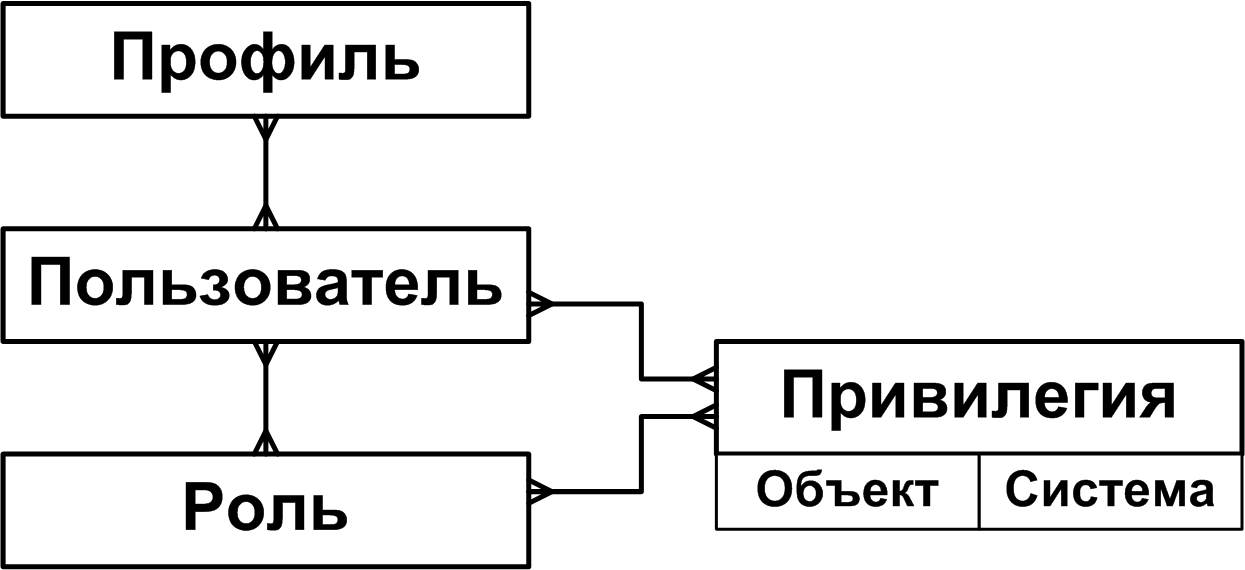
\includegraphics[height=.5\textheight]{pict/oracle} }
        \mode<article>{ 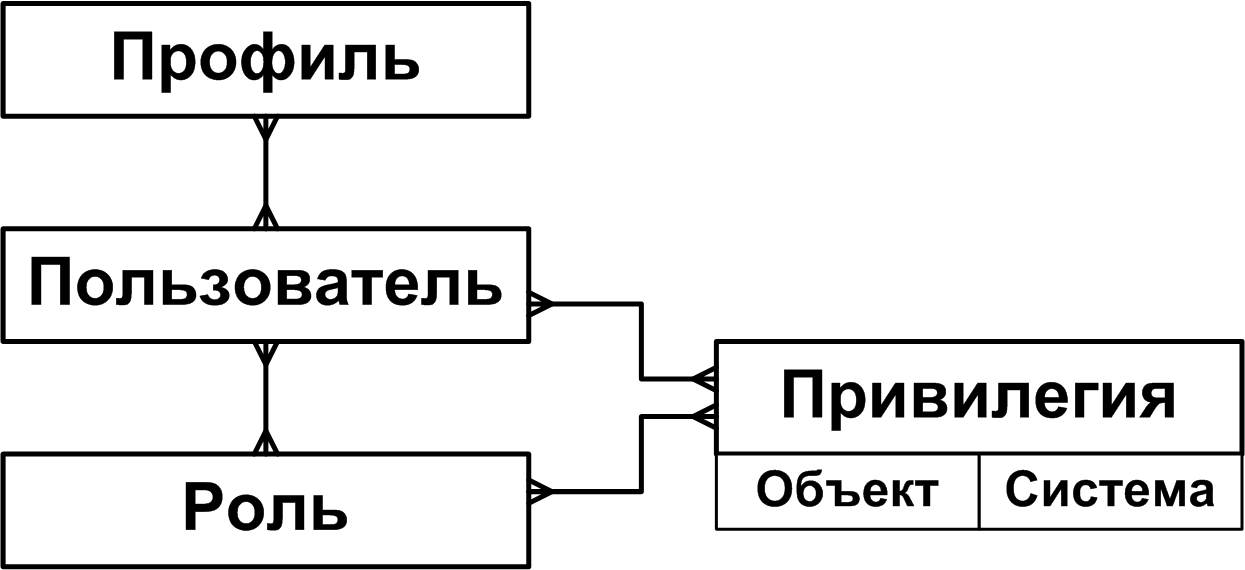
\includegraphics[width=.7\textwidth]{pict/oracle} } 
        \caption{Безопасность в ORACLE}\label{pict:oracle}
    \end{center}
\end{figure} 
\mode<article>{см. рис. \ref{pict:oracle}}
\end{frame}


\begin{frame}
    \frametitle{ORACLE}
    
    \begin{itemize}
        \item С \alert{пользователем} может быть ассоциировано множество \alert{профилей}, \alert{ролей} и 
                \alert{привилегий}.
                
        \item \alert{Профиль} определяет объем доступных пользователю системных ресурсов.
        \begin{itemize}
            \item Процессорное время, длительность подключения, количество параллельных подключений, и т.д.
        \end{itemize}
        
        \item \alert{Роль} --- абстрактный субъект, с которым может быть ассоциировано множество \alert{привилегий}.
        
        \item \alert{Привилегии} определяют возможности. Разделяются на два типа.
        \begin{itemize}
            \item \alert{Объектные} определяют доступ в отношении конкретных объектов базы данных: таблиц, 
                представлений, индексов и т.д.
                
            \item \alert{Системные} определяют возможные действия над СУБД с использованием команд. Например, создание / удаление / модификация таблицы, пользователя, сессии и т.д.
        \end{itemize}
    \end{itemize} 
\end{frame}


\appendix


%раскрыть тему в будущем
\begin{frame}
    \frametitle{Каналы утечки}

    Даже в системе, в основу которой положена математически обоснованная (формальная) модель контроля доступа. Могут происходить утечки.
    \begin{itemize}
        \item В результате действий инсайдера с большими полномочиями.
        \item Организация тайных каналов утечки информации.
        \begin{itemize}
            \item Использование стеганографических методов (например, тайная передача данных, сокрытых в файлах изображений или звуковых файлах).
            \item Модуляция на основе общедоступных объектов (нагрузка процессора, ошибки отсутствия страниц в памяти, блокировка файлов, и т.д.).
        \end{itemize}
    \end{itemize}
\end{frame}


\begin{frame}
    \frametitle{Объектно-ориентированное программирование}
    \framesubtitle{Система контроля доступа на примере паттерна <<одиночка>>}
    \begin{example}[Singleton]
        Класс имеет только один экземпляр и обеспечивает глобальный доступ к нему.
    \end{example}
\end{frame}


\begin{frame}[fragile]
    \frametitle{Объектно-ориентированное программирование}
    \framesubtitle{Система контроля доступа на примере паттерна <<одиночка>>}
\begin{semiverbatim}
\uncover<1->{\alert<0>{class Singleton \{ }}
\uncover<2->{\alert<2>{public:     static Singleton& \alert{Instance}() \{ }}
\uncover<3->{\alert<3>{                if (!pInstance_) }}
\uncover<3->{\alert<3>{                    pInstance_ = new Singleton(); }}
\uncover<3->{\alert<3>{                return *pInstance_; }}
\uncover<2->{\alert<2>{            \} }}
\uncover<5->{\alert<5>{            void foo() \{...\} //Не статические  }}
\uncover<5->{\alert<5>{                             //член-функции и член-данные! }}
\uncover<3->{\alert<3>{private:    static Singleton *pInstance_ = 0; }}
\uncover<4->{\alert<4>{            Singleton(); }}
\uncover<4->{\alert<4>{            Singleton(const Singleton&); }}
\uncover<4->{\alert<4>{            Singleton& operator=(const Singleton&); }}
\uncover<4->{\alert<4>{            ~Singleton(); }}
\uncover<1->{\alert<0>{\} }}
\end{semiverbatim}
\end{frame}


\begin{frame}[fragile]
    \frametitle{Объектно-ориентированное программирование}
    \framesubtitle{Система контроля доступа на примере паттерна <<одиночка>>}
\begin{semiverbatim}
    Singleton::Instance().foo();             //allowed
    
    Singleton s1;                            //\alert{denied}
    Singleton s2(Singleton::Instance());     //\alert{denied}
    Singleton s3=Singleton::Instance();      //\alert{denied}
    Singleton *ps = new Singleton();         //\alert{denied}
    
    Singleton *ps1 = &Singleton::Instance(); //allowed
    delete ps1;                              //\alert{denied}
\end{semiverbatim}
\end{frame}

%сводка по ссылкам
\begin{frame}
    \frametitle{Источники}
    
    \begin{itemize}
        \item О системах контроля доступа доступно изложено в \cite{bib:tannen:os}.
    
        \item Формальные модели безопасности см. в \cite{bib:zegzda:secbase}.

        \item О безопасности в Unix см. \cite{bib:robachevsky:unix}. 
    
        \item О безопасности в Windows см. \cite{bib:russinovich:wininternals}. 

        \item О паттернах программирования см. \cite{bib:gamma:patterns}. 
        
        \item О Singleton в C++ исчерпывающе в \cite{bib:alexandrescu:moderncpp}.
    \end{itemize}
\end{frame}


\begin{frame}[allowframebreaks]{Библиография}
    \bibliographystyle{gost780u}
    \bibliography{./../bibliobase}
\end{frame}


\end{document}